 \section{Results}\label{sec:results}
 To extract the signal strength from all the four sub channels, a combination template fit was applied.
 This fit concentrate also makes use of $X_B-X_C$ distribution in each channel. 
 The combined log-likelihood is defined as the sum of that in each sub channel.
 The free parameters are the same as that in the fit of each channel, described in \ref{subsec:flavortagging}. 
 The fraction of each flavor are set as common parameter,while the over all hadronic yields in each channel are set as indepedent parameter. The combined fit results are shown in figure \ref{fig:combined_fit}. 
 
\begin{figure}[!htpb]
\label{fig:combined_fit}
\centering
\subfigure[]
{
  \begin{minipage}[b]{0.31\textwidth}
  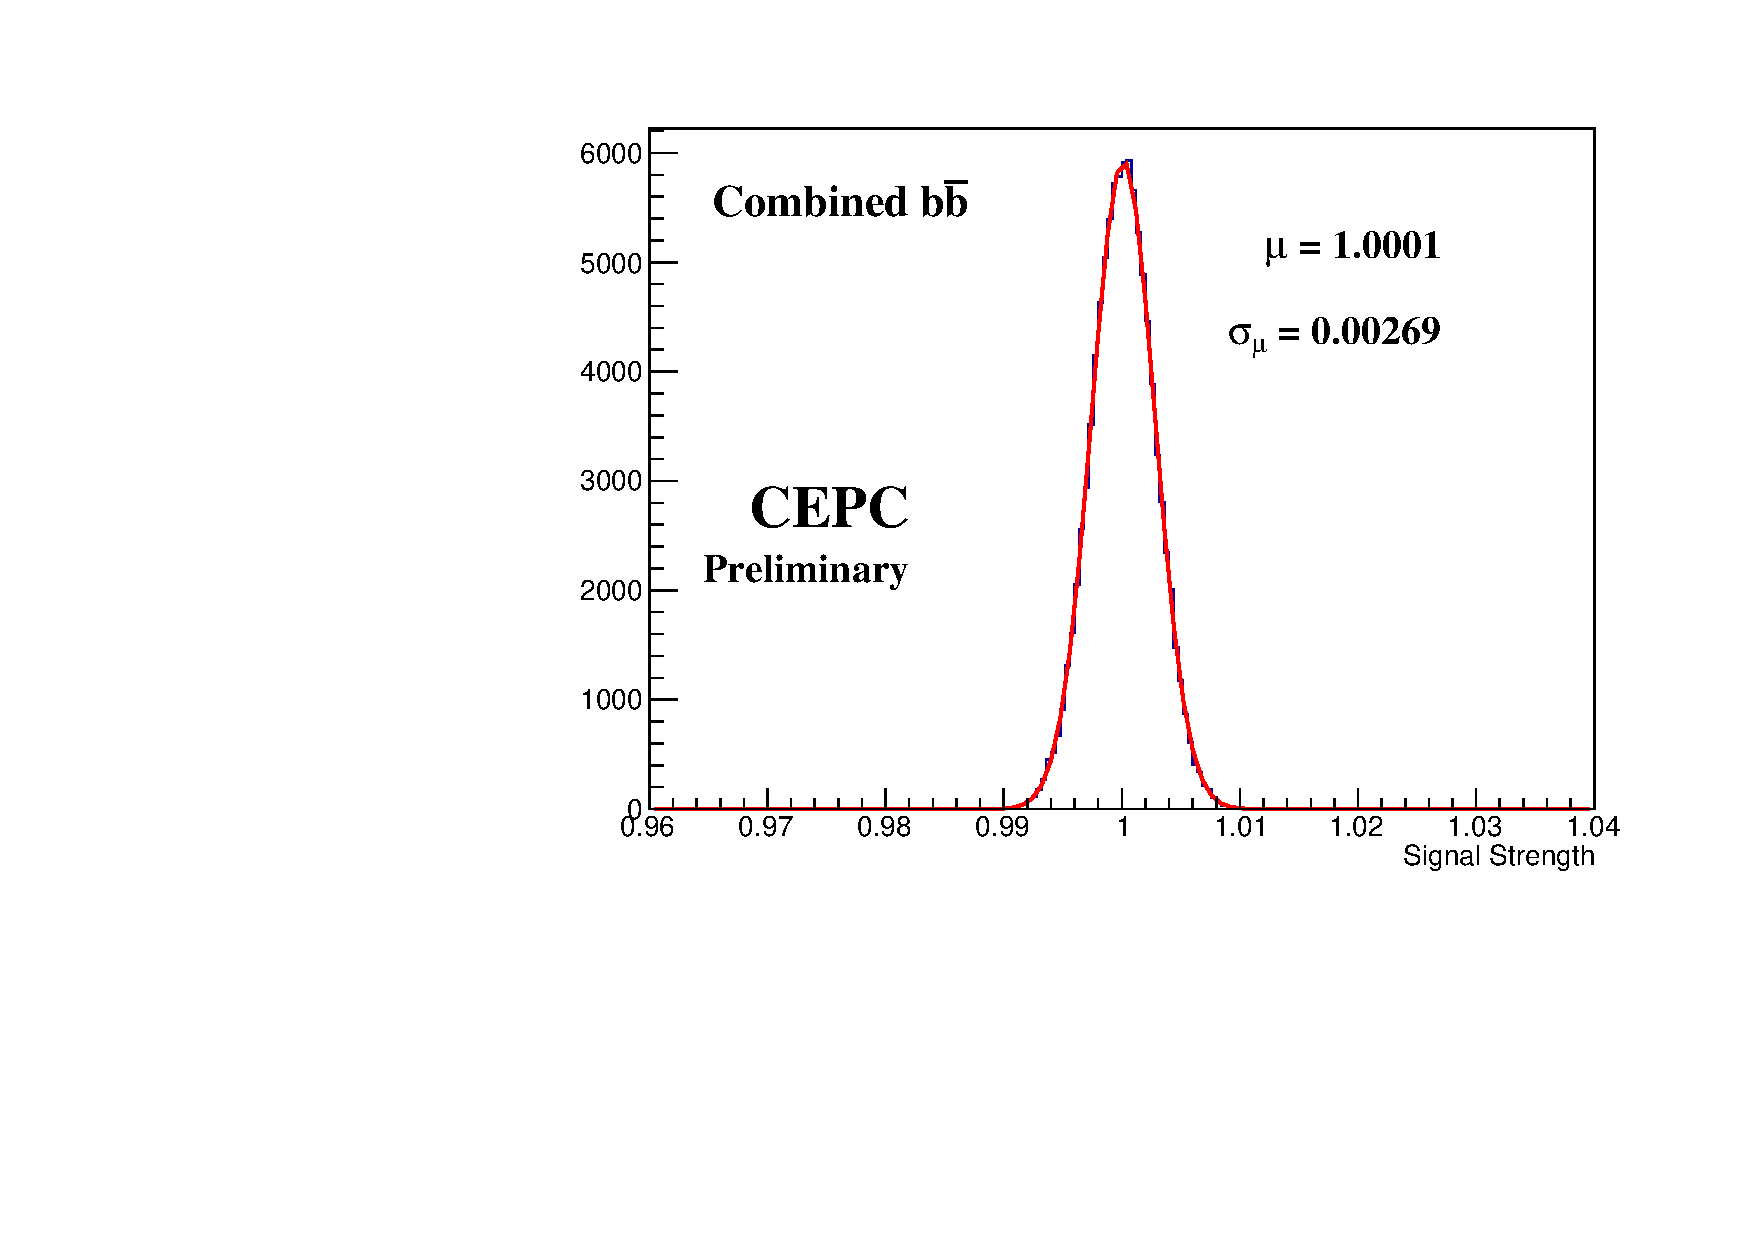
\includegraphics[width=\textwidth]{Template/toymc_combined_bb.pdf}
  \end{minipage}
}
\subfigure[]
{
  \begin{minipage}[b]{0.31\textwidth}
  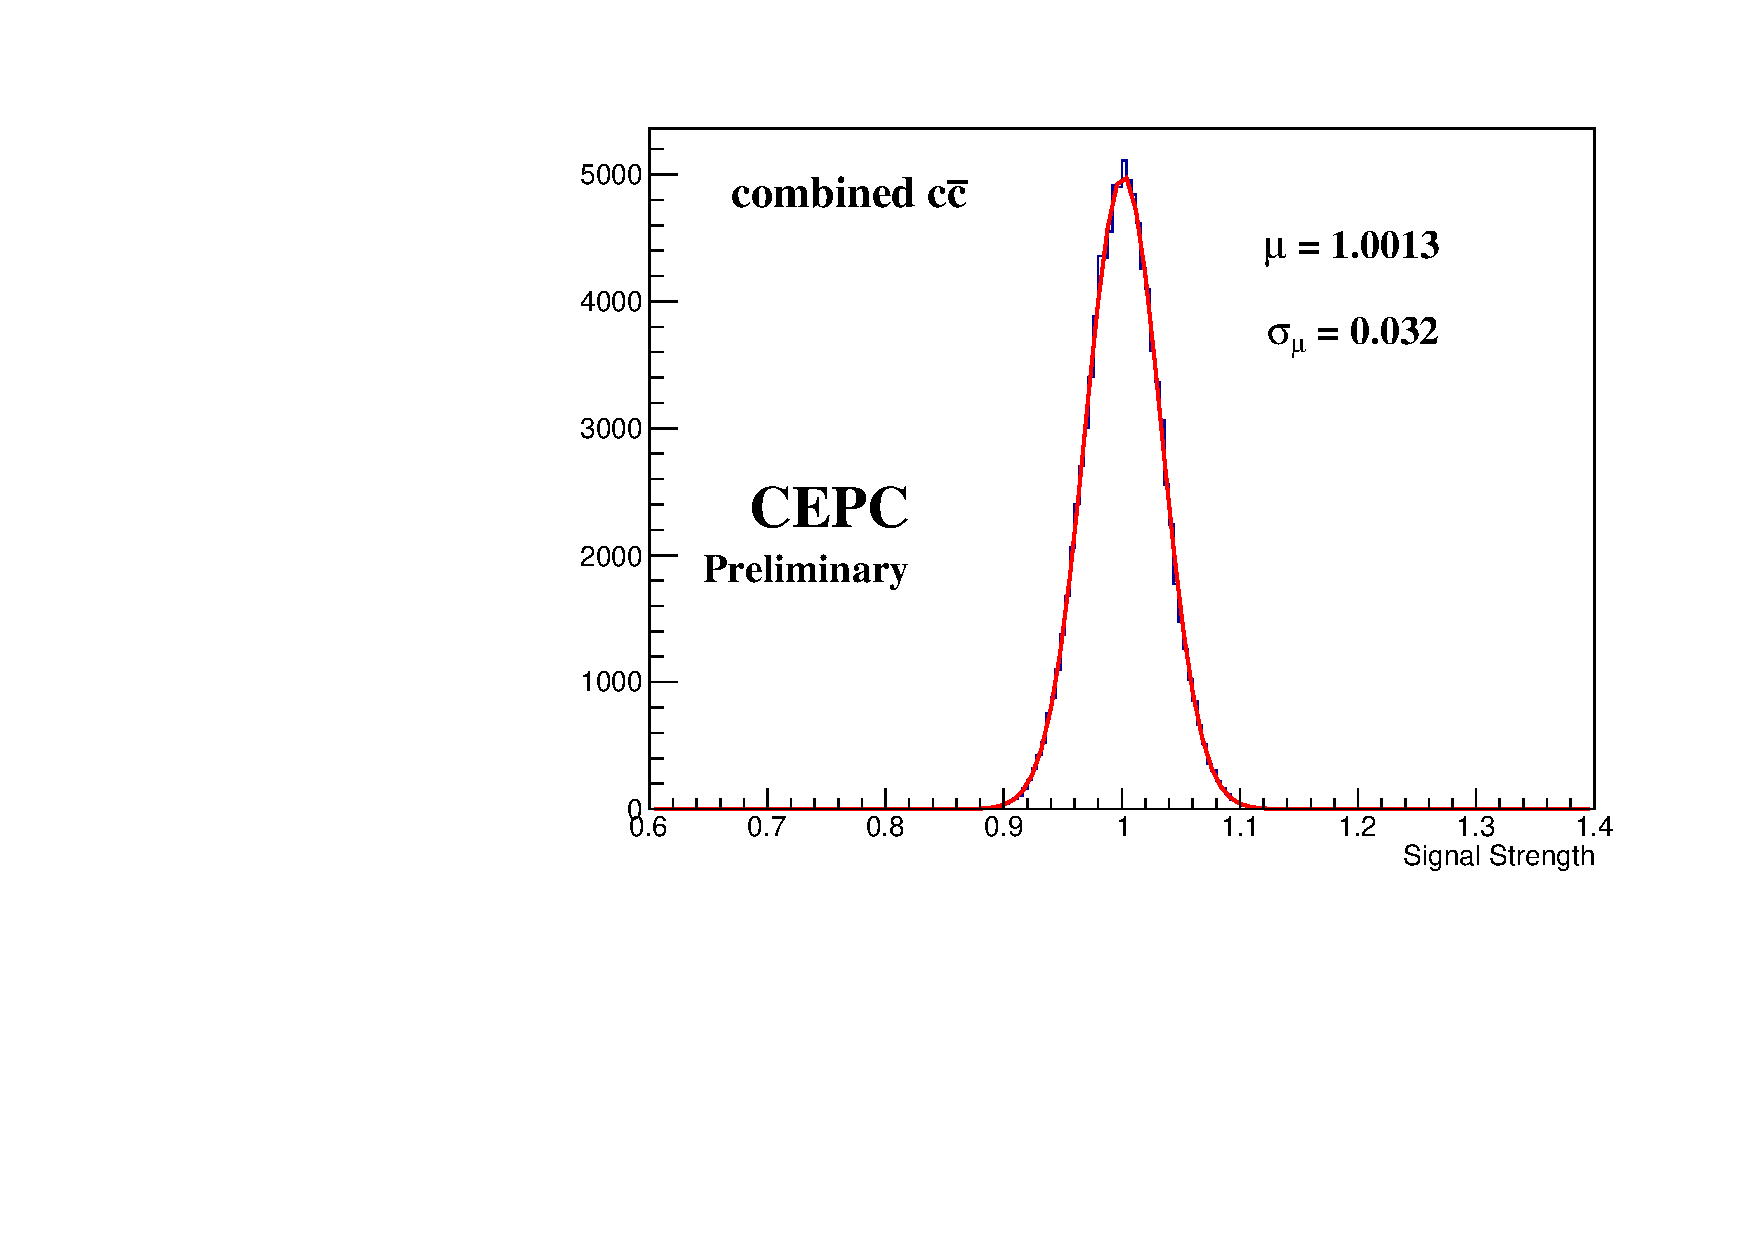
\includegraphics[width=\textwidth]{Template/toymc_combined_cc.pdf}
  \end{minipage}
}
\subfigure[]
{ 
   \begin{minipage}[b]{0.31\textwidth}
   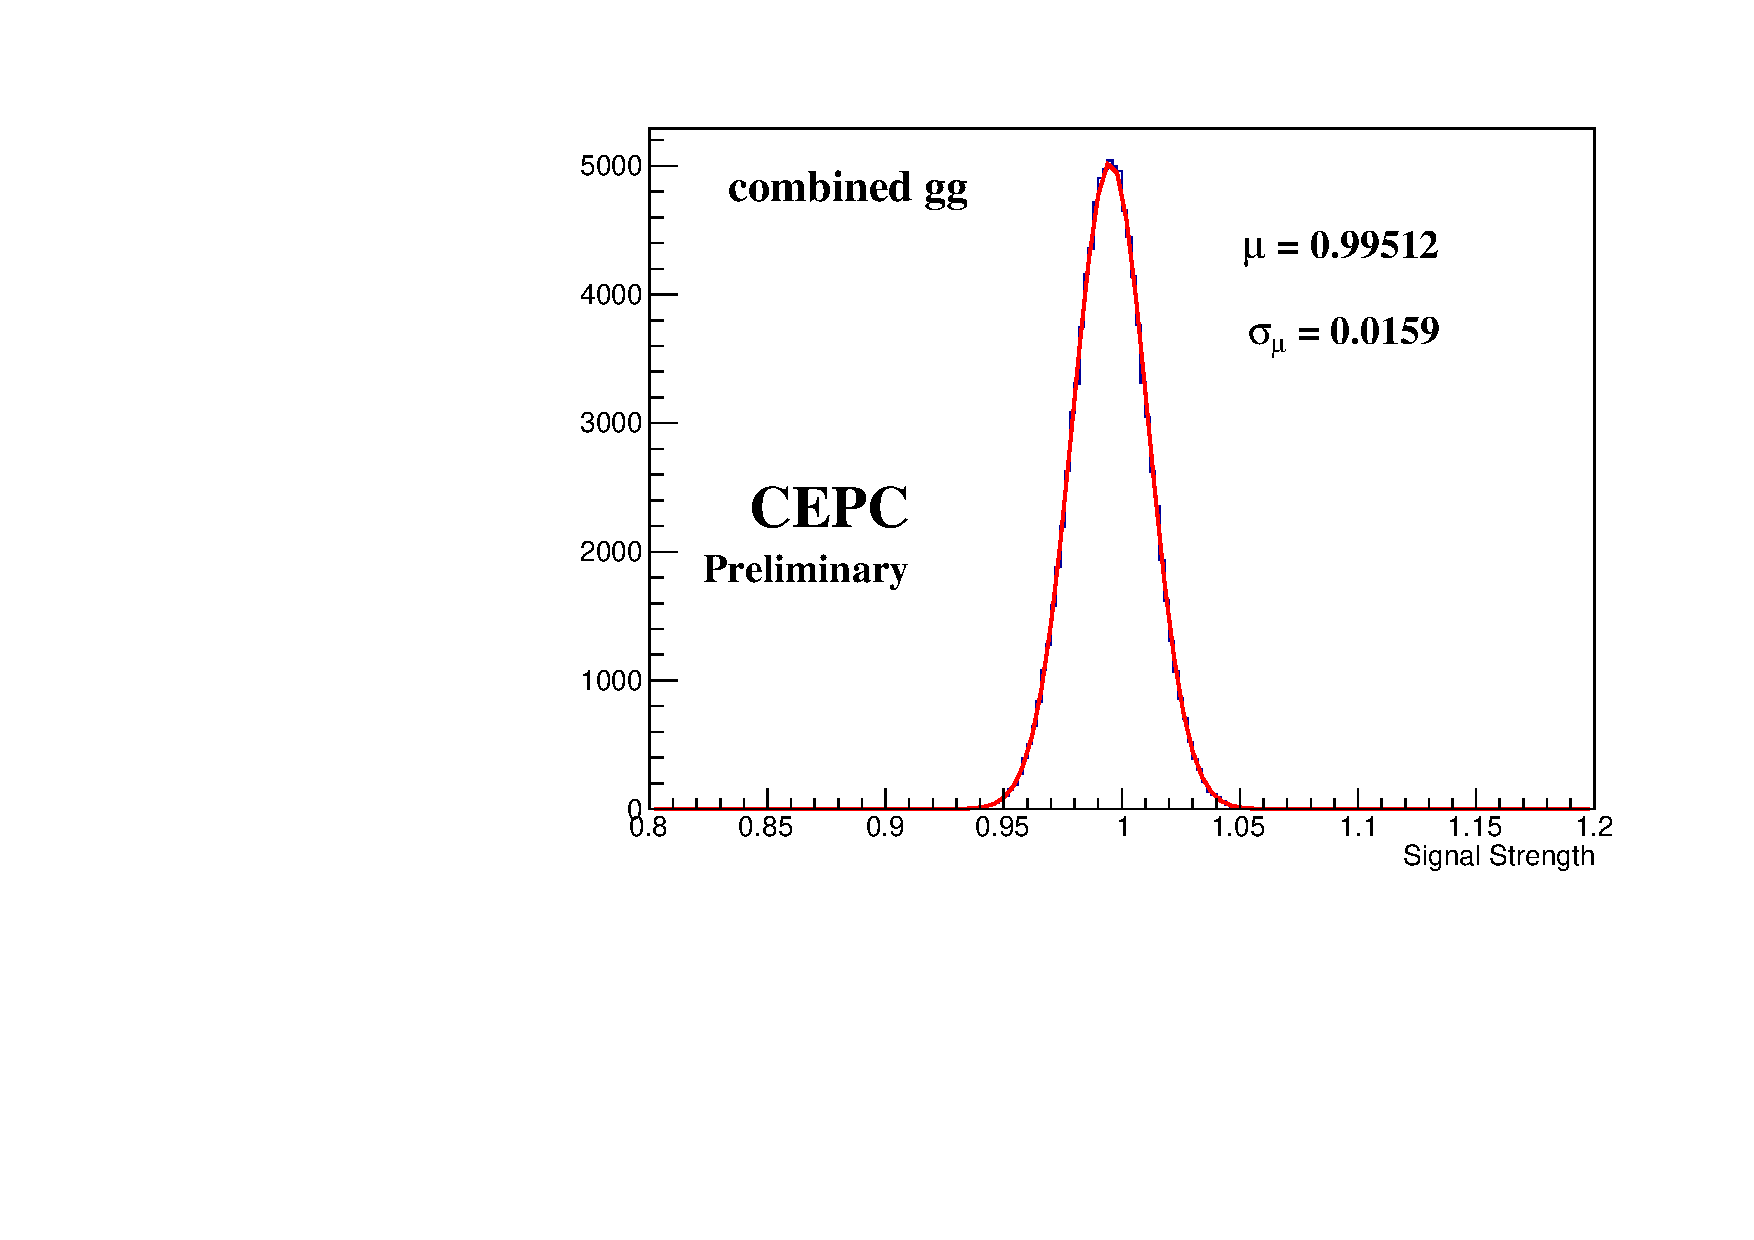
\includegraphics[width=\textwidth]{Template/toymc_combined_gg.pdf}
   \end{minipage}
}
\caption{Combined template fit results of signal strength for $H\rightarrow \bpair$, $H\rightarrow\cpair$ and $H\rightarrow\gpair$ process.}
\end{figure}
 
%After the cutflow(except for the $\chi^2$ cut in the last step) being applied, the template fit was implemented to the sample consist of $qqH\to bb/cc/gg$ and the background events. The fast simulation background sample don't have vertex reconstructed so there is no way to apply flavor tagging on it. Thus currently the background only contains the fully reconstructed  higgs production sample, including 75413 $\qqbar\Hboson\to\qqbar\Wboson\Wboson$ events, 10091 $\qqbar\Hboson\to\qqbar\Zzero\Zzero$ events, 8444 $\qqbar\Hboson\to\qqbar\tautau$ events and 7780 $\nnbar\Hboson\&\leplep\Hboson$ events. The fitted sample distribution in $X_B-X_C$ coordinate is shown in figure \ref{fig_data}. The fitting result is shown in table \ref{tab:fit_result}
%\begin{figure}[!htpb]\label{fig:fit_data}
%\centering
%    \includegraphics[width=0.88\textwidth]{figures/c1_n2.eps}
%\caption{ Distribution of $X_B-X_C$ fitted sample}
%\label{fig:templates}
%\end{figure}
%
%\begin{table}[h]
%\begin{center}
%\begin{tabular}{cccccccc}
%\hline
%\hline
%Channel		&	data	&	fit	&	sigma	&	sigma/fit&	bias	&	bias/data	&	template	\\
%\hline
%$\bbbar$	&	263.5k	&	261.2k	&	699	&	0.266\%	&	2357	&	0.894\%		&	data itself	\\\hline
%$\ccbar$	&	12.22k	&	12.95k	&	574	&	4.43\% 	&	737	&	6.03\%		&	data itself	\\\hline
%gg		&	41.06k	&	45.93k	&	1359	&	2.96\% 	&	4875	&	11.9\%		&	data itself	\\\hline
%\multirow{2}{2cm}{$\ffbar\Hboson$ background}&\multirow{2}{*}{102.5k}&\multirow{2}{*}{99.28k}&\multirow{2}{*}{2069}&\multirow{2}{*}{2.08\% }&\multirow{2}{*}{-3255}&\multirow{2}{*}{-3.18\%}&\multirow{2}{*}{\minitab[c]{$\nnbar\Hboson\&\qqbar\Hboson$:data itself \\ the others: other events}} \\\\
%\hline
%\hline
%\end{tabular}
%\caption{Template fit results, and the deviation to the true value}
%\end{center}
%\label{tab:fit_result}
%\end{table}
%The outcome of the fit shows significant deviation from true event yields for $H\to gg$ and $ffbarH$, while 
%the fitted $H\to bbar$ and $H\to ccbar$ event yields is relatively reasonable.  Strong correlation between $H\to gg$ and $ffH$ from fitting can be found in table \ref{tab:fit_matrix}, largely due to resemblance between the distribution of these two process shown in bottom plots in figure \ref{fig:templates} and cause considerable deviation in the fitting. Thus a predetermination of the $ffH$ fraction can significantly reduce the uncertainty of $H \to gg$ fraction from fitting.
%\begin{table}[h]
%\begin{center}
%\begin{tabular}{|c|c|c|c|c|c|c|c|}
%\hline
%\hline
%Channel	&	$\bbbar$	&	$\ccbar$	&	$gg$		&	$\ffbar\Hboson$\\\hline
%$\bbbar$	&	1.000	&	0.280  	&	0.332	&	-0.453		\\\hline
%$\ccbar$	&	0.280  	&	1.000  	&	0.629 	&	-0.774		\\\hline
%$gg$		&	0.332  	&	0.629  	&	1.000 	&	-0.927		\\\hline
%$\ffbar\Hboson$&0.453 	&	-0.774	&	-0.927  	&	1.000		\\\hline
%\hline
%\hline
%\end{tabular}
%\caption{Template fit correlation matrix}
%\end{center}
%\label{tab:fit_matrix}
%\end{table}
